\documentclass{article}
\usepackage{graphicx}
\usepackage{float}
\usepackage[margin=.75in]{geometry}

\begin{document}

Code used in production of plots for this section can be found at https://github.com/cfmcginn/SystBio/tree/master/HW5.
\section{2.d}

Plotted are the stochastic simuations in Fig.~\ref{fig1}, the corresponding long time integral of counts in Fig.~\ref{fig2}, and the overlay of a system where X represses its own synthesis in Fig.~\ref{fig3}. Note that B was chosen to be 200 to match the condition that the steady state value match system A when A = 100. Note that Poissonion distribution is a close match by eye, but fails a chi-square because of the relation between successive numbers of counts in the long time integral. Also note that in Fig.~\ref{fig3} the self-repressing X has lower fluctuations in stochastic simulation.

\begin{figure}[H]
    \centering
    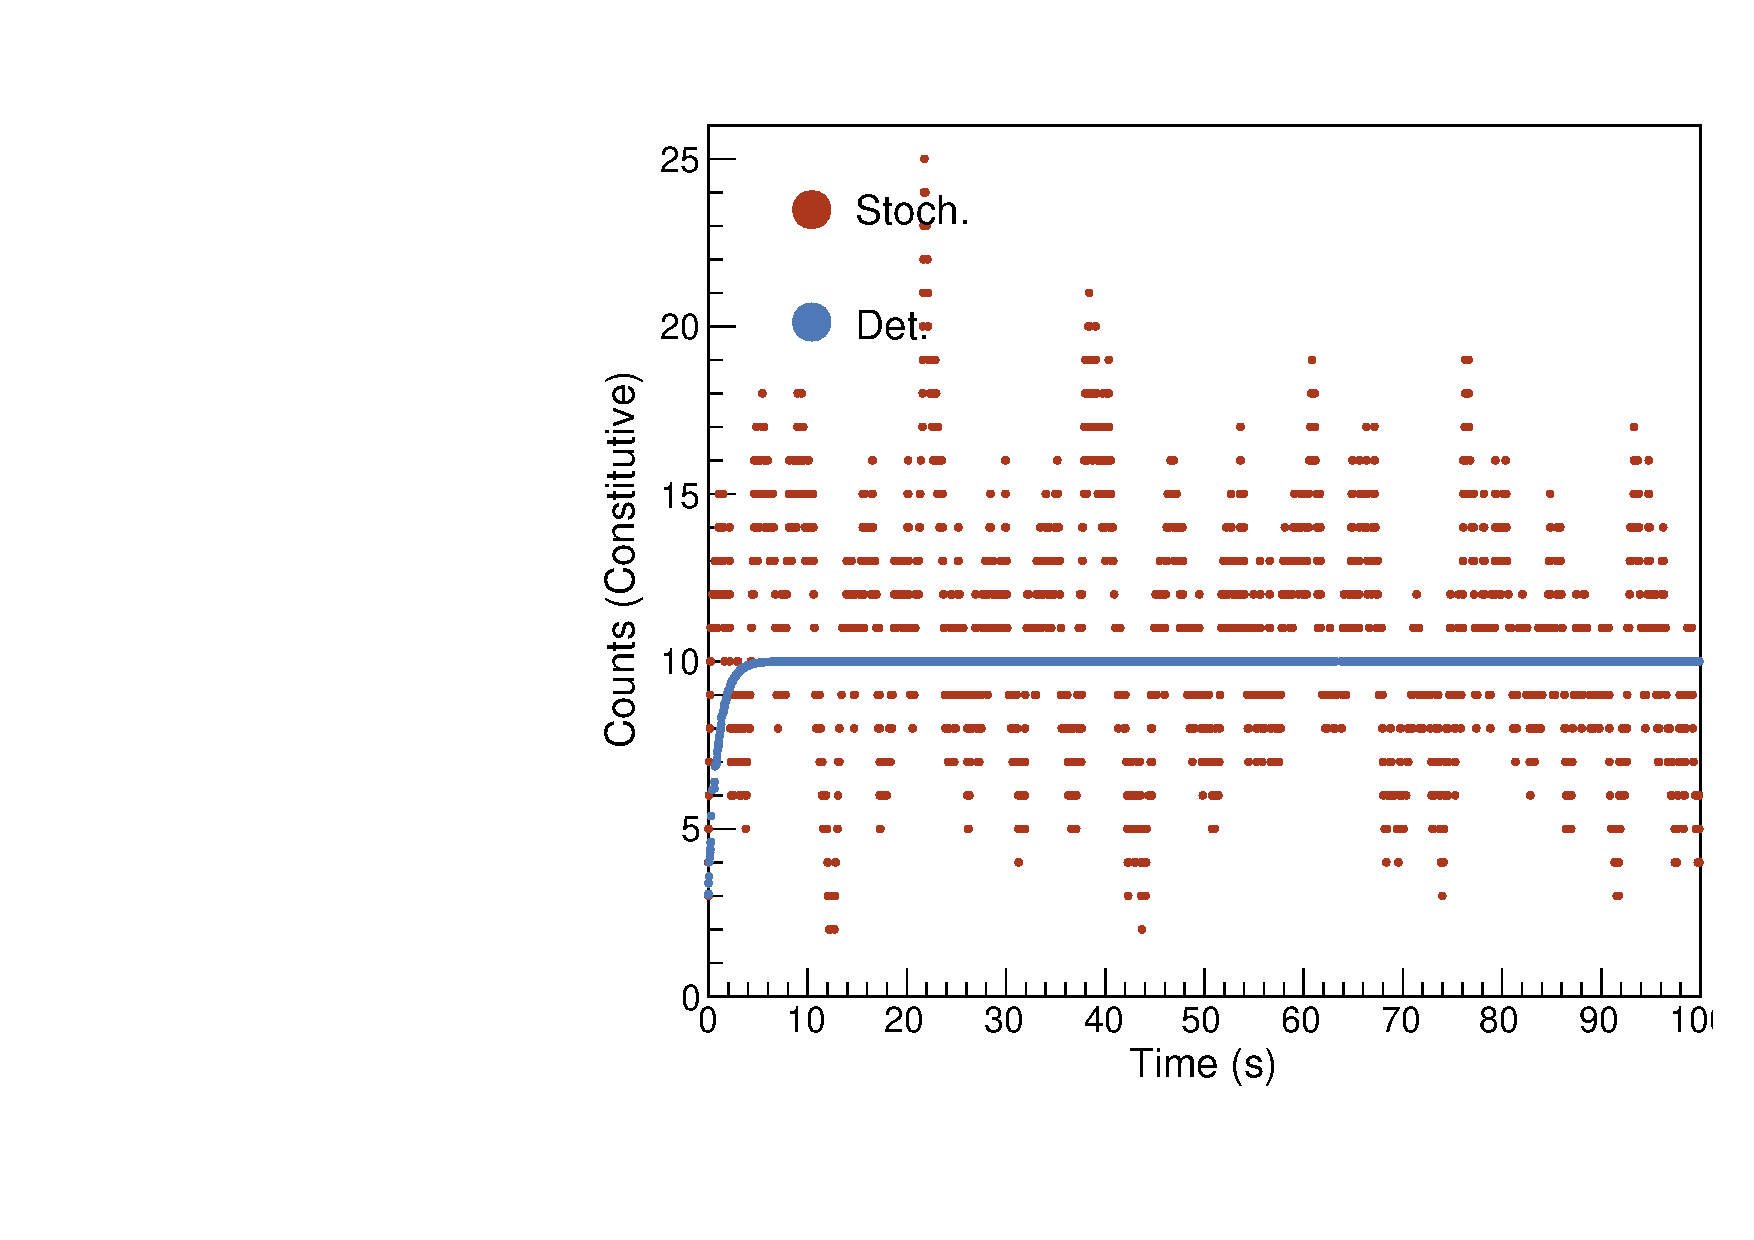
\includegraphics[width=.49\textwidth]{canv10.pdf} 
    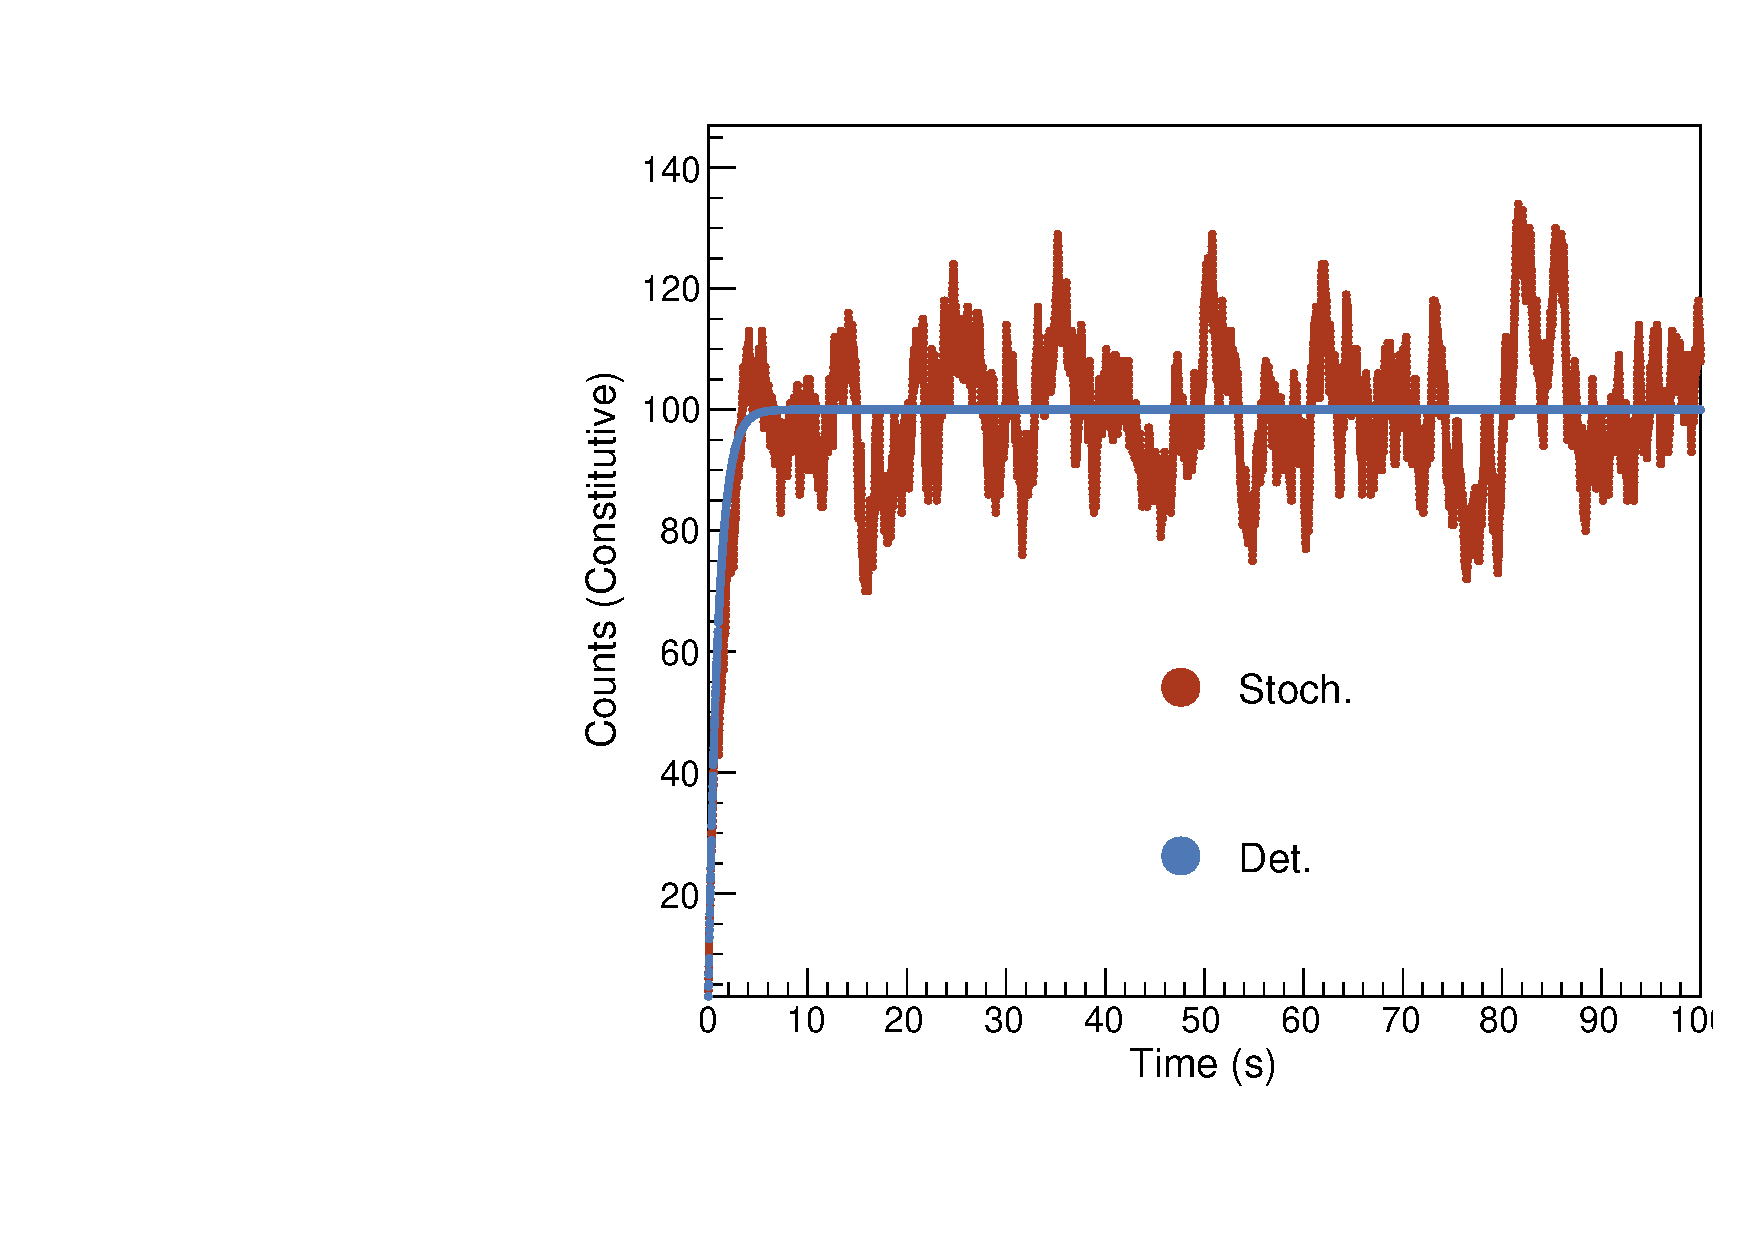
\includegraphics[width=.49\textwidth]{canv100.pdf} 
    \caption{Stochastic simulation thru 100 seconds of system A. Left is A = 10, Right is A = 100. The overlaid blue is the corresponding behavior of the deterministic system.}
    \label{fig1}
\end{figure}

\begin{figure}[H]
    \centering
    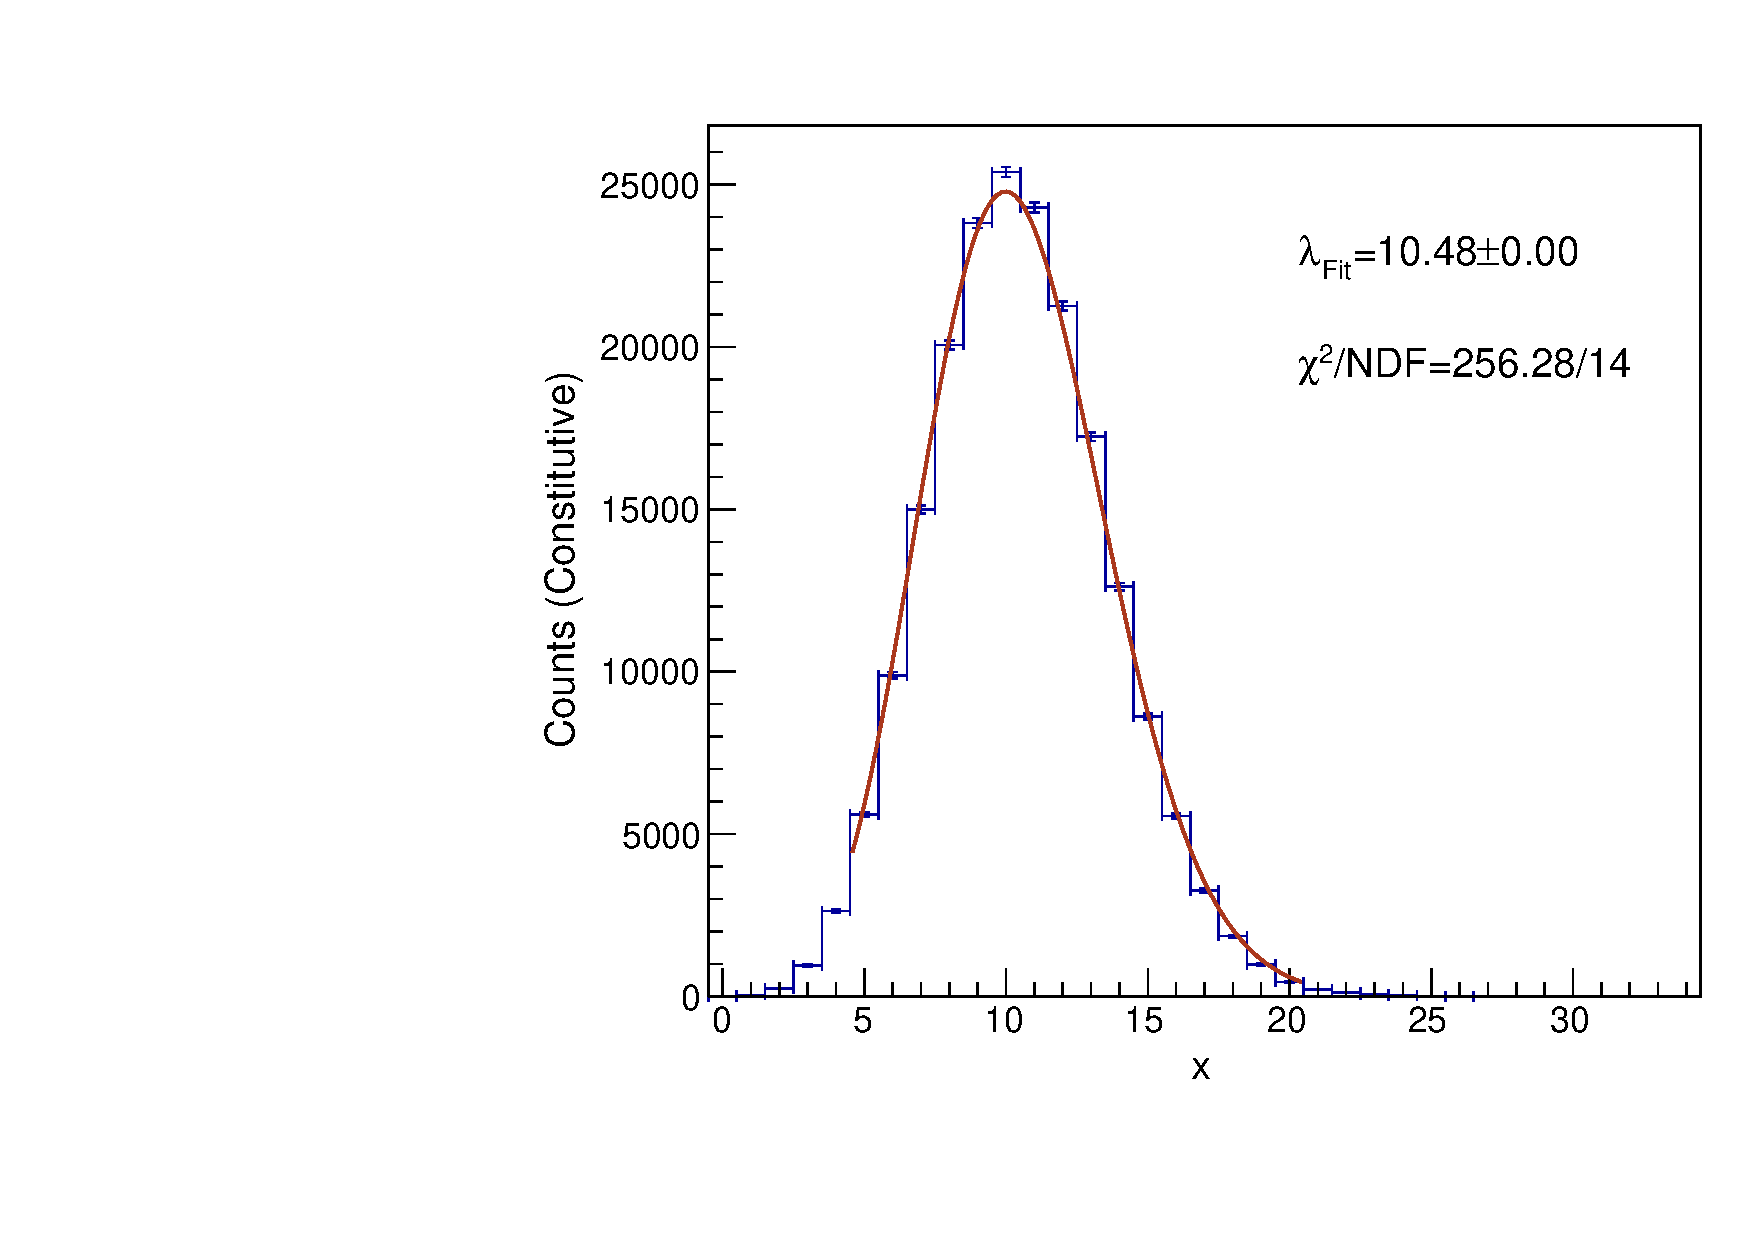
\includegraphics[width=.49\textwidth]{canv10_2.pdf} 
    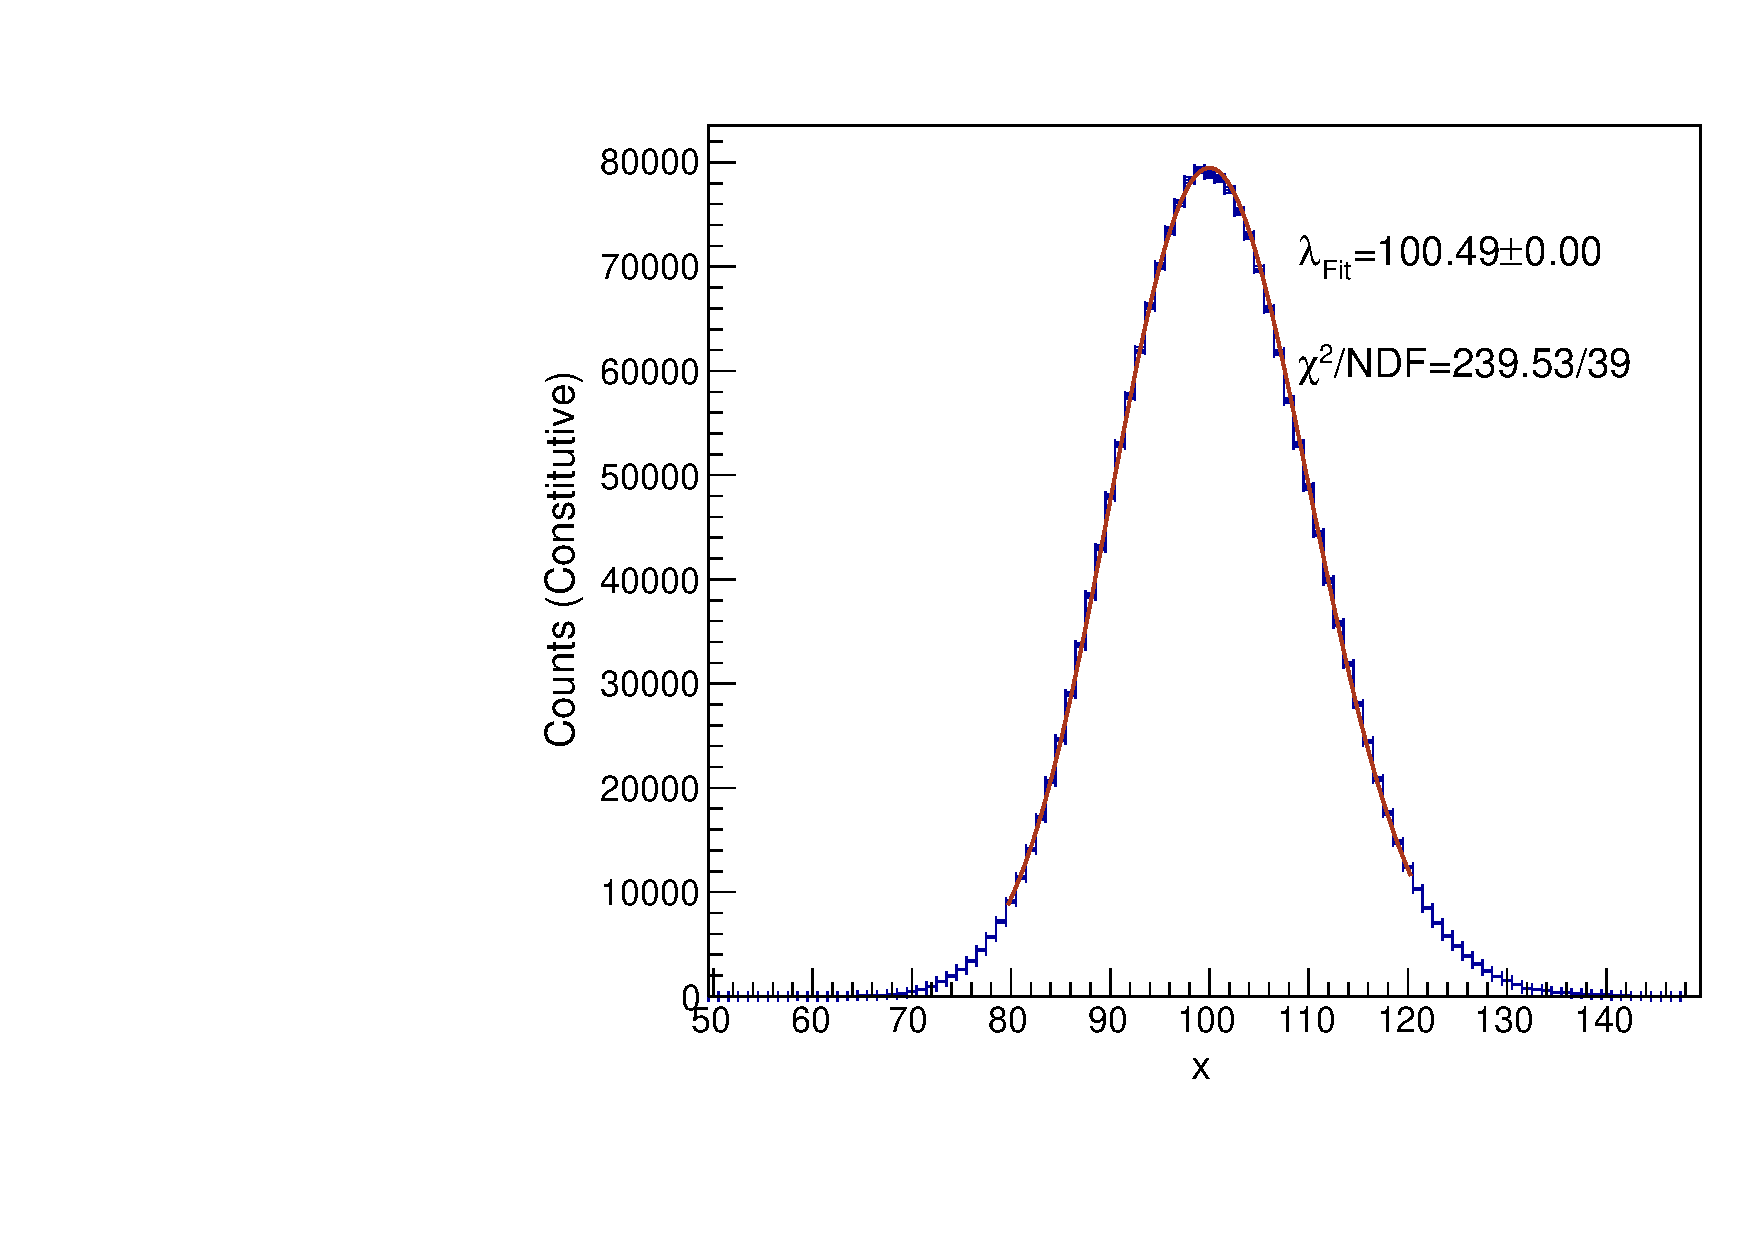
\includegraphics[width=.49\textwidth]{canv100_2.pdf} 
    \caption{Long time integral of the number of counts in system A. Left is A=10, right is A=100. Note that while by eye the two seem to map nicely onto a Poissonion, a chi-square test shows they deviate somewhat significantly. This is because on the long time integral, the number of counts from one time-step to another are related (n plus or minues one). True poissonion statistics requires the counts to be memoryless.}
    \label{fig2}
\end{figure}

\begin{figure}[H]
    \centering
    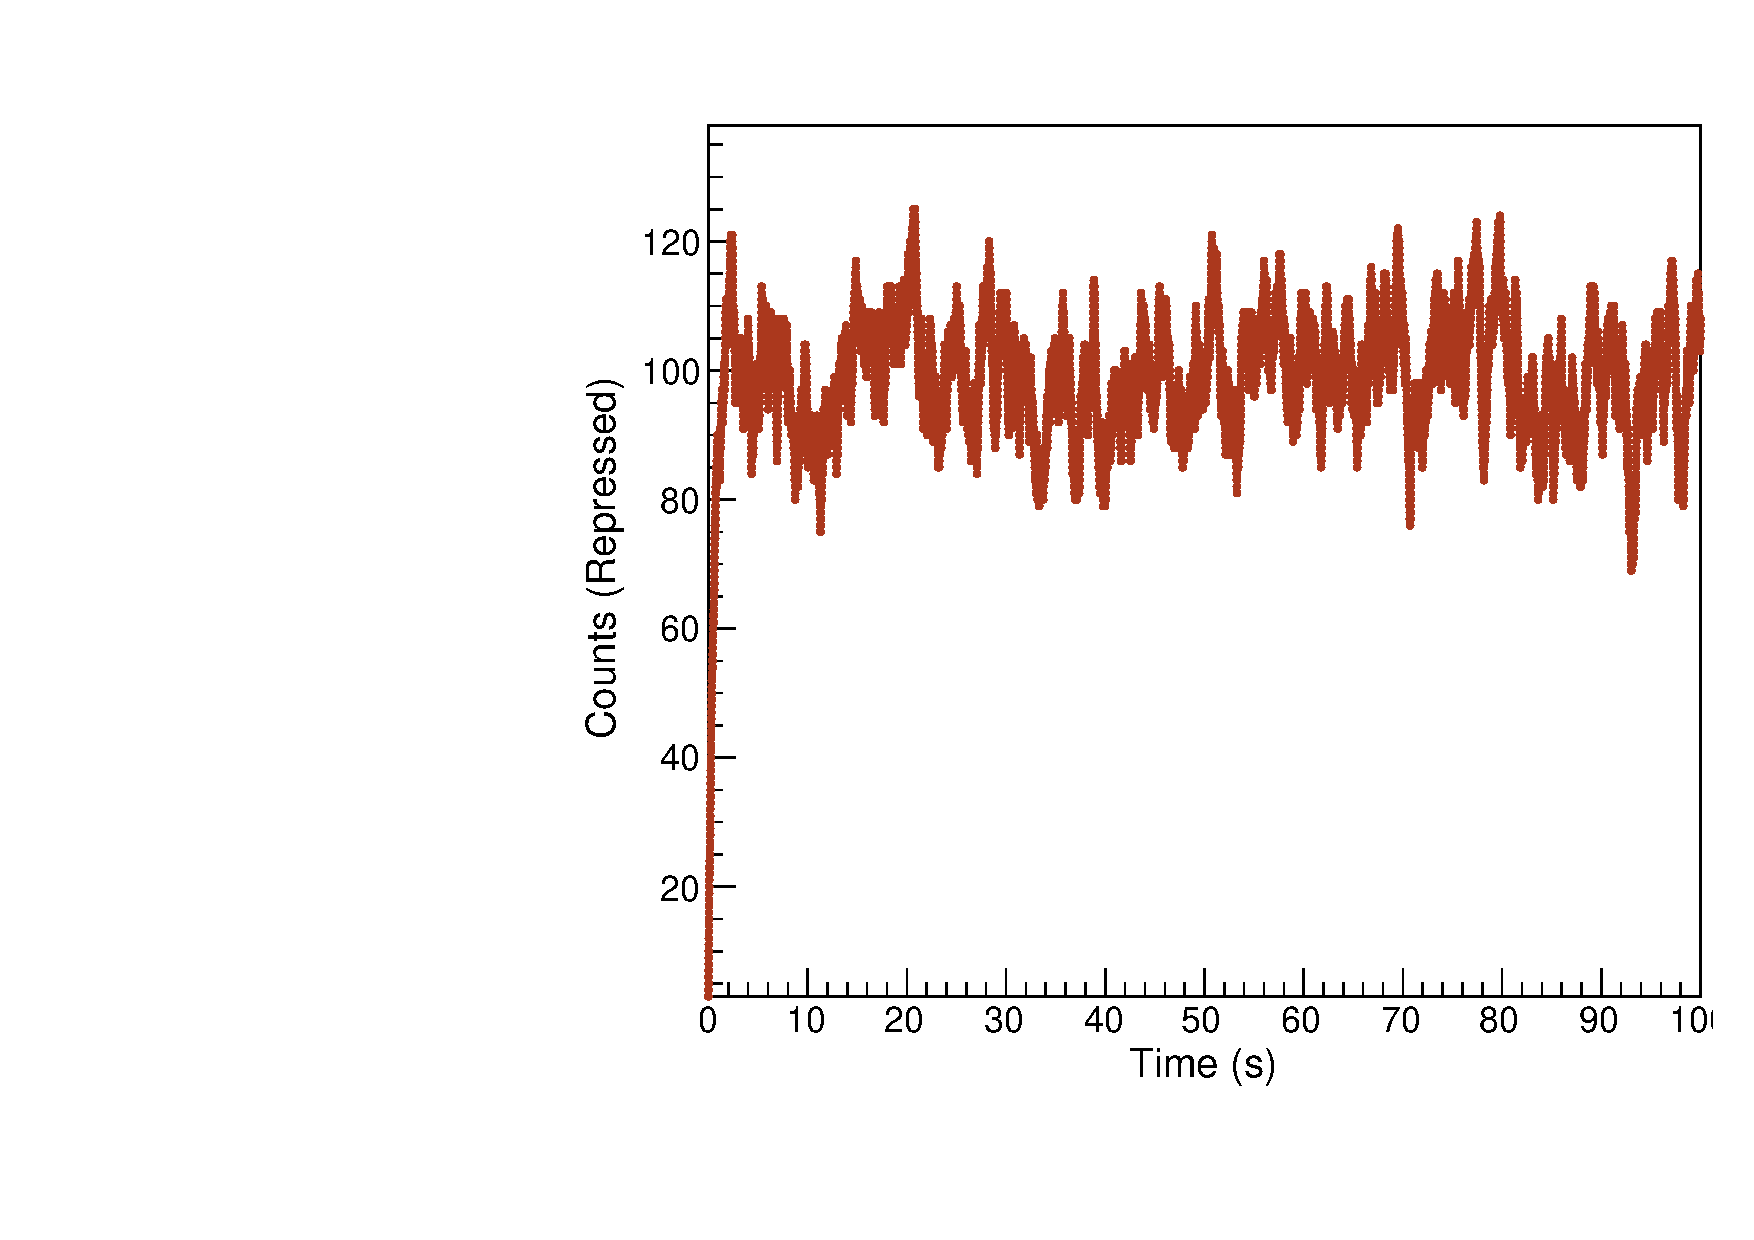
\includegraphics[width=.49\textwidth]{canv100K.pdf} 
    
    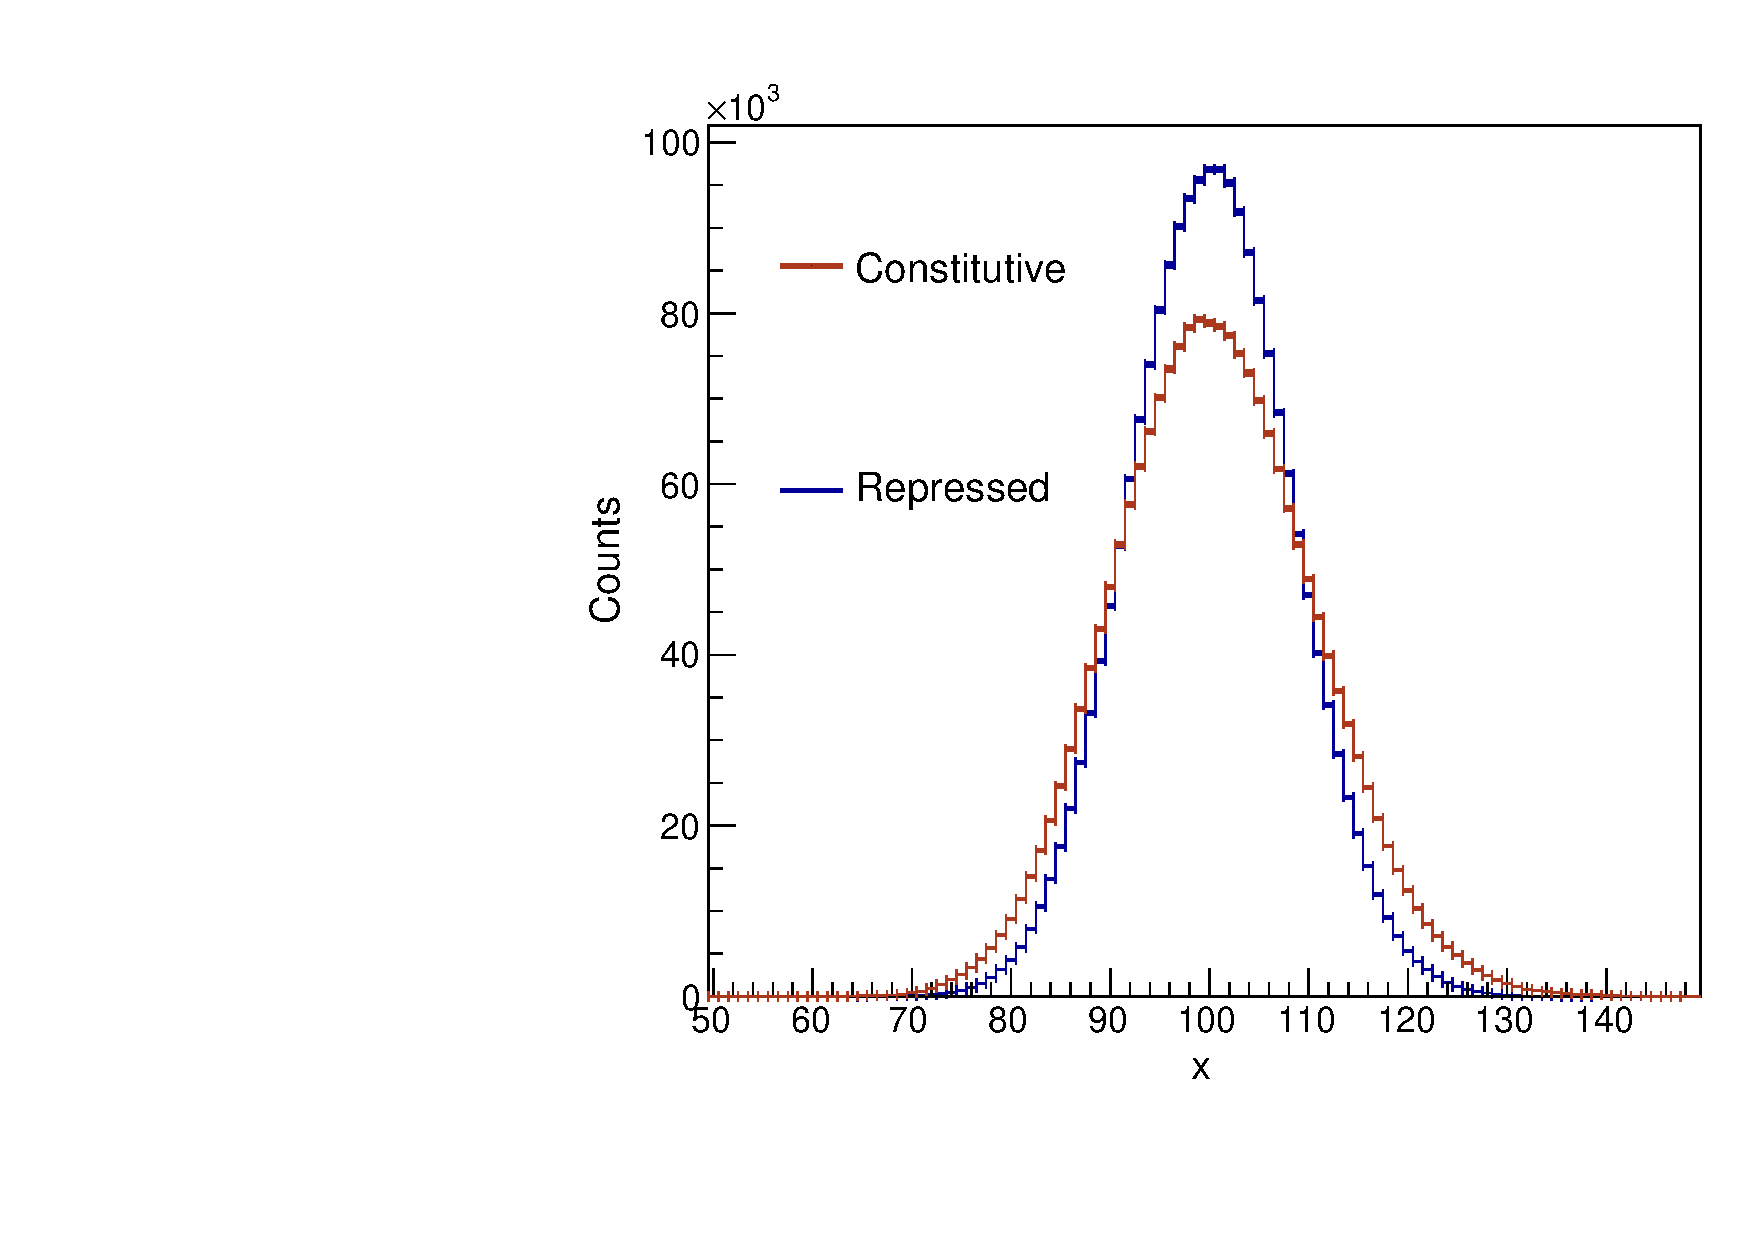
\includegraphics[width=.49\textwidth]{canv100K_2.pdf} 
    \caption{Distribution of constitutive and self-repressing X. Self-repression results in a much narrower distribution of steady-state counts in the long time integral. Left-hand side also shows faster rise behavior of the self-repressing X.}
    \label{fig3}
\end{figure}

\section{4.f-h}

Fig~\ref{fig4} shows the bistable system simulated thru five thousand seconds. There are clearly two states of stability, the state centered around 19 and the state centered around 130. The crossing point between the two states is 50, or the location of the unstable fixed point separating the two. The fraction of time between the two states is estimated by counting the number of seconds the system is below 50 and the number of seconds the system is above 50. For this simulation we get 1189.42 seconds below 50 and 3810.59 seconds above 50, giving probabilities of .238 and .762 for each state. By taking the simulation to much larger times we can get a more exact measure of the relative probabilities. From one million seconds, the relative probability is .197 and .803.


\begin{figure}[H]
    \centering
    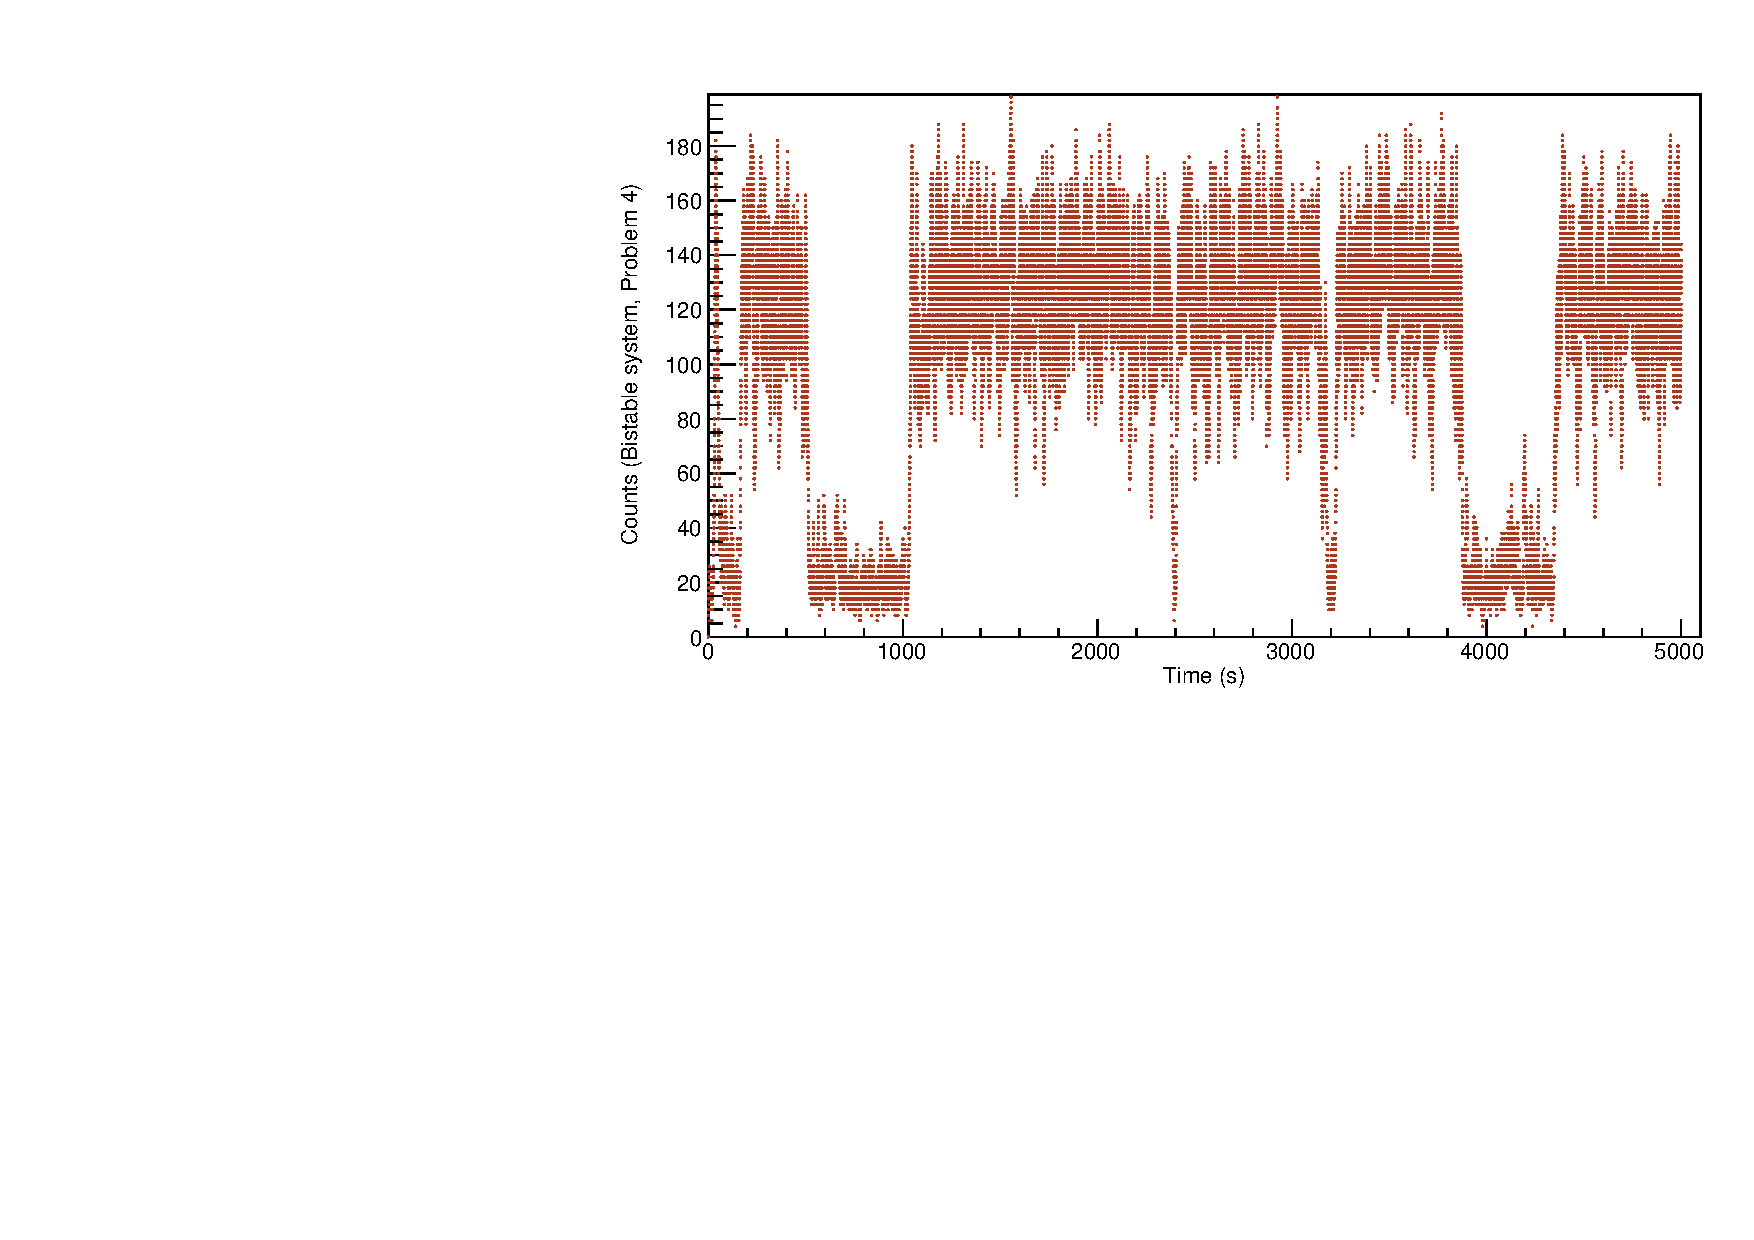
\includegraphics[width=.99\textwidth]{canvBistableGil_Final.pdf} 
    \caption{Simulation of the bistable system using the Gilespie method thru 5000 seconds. The two stable states of the system are separated by 50, with central values of roughly 19 and 130.}
    \label{fig4}
\end{figure}

Fig~\ref{fig5} shows the potential exponentiated, the denominator f(n) + g(n), and the probability before normalization. Clearly the dominant behavior is the exponentiated potential which defines the two peak probability values, with the denominator only dropping the probability of the 130 peak. Normalization requires dividing points by 1.74706e+10, a value for A inverse. After this division we recover Fig.~\ref{fig6}, matching expectations. Integrating Fig.~\ref{fig6} from 0 to 50 and 50 to infinity gives expected time in each stable state of .194 and .806, respectively, roughly consistent with our stochastic simulations at the limit of large time (one million seconds).

\begin{figure}[H]
    \centering
    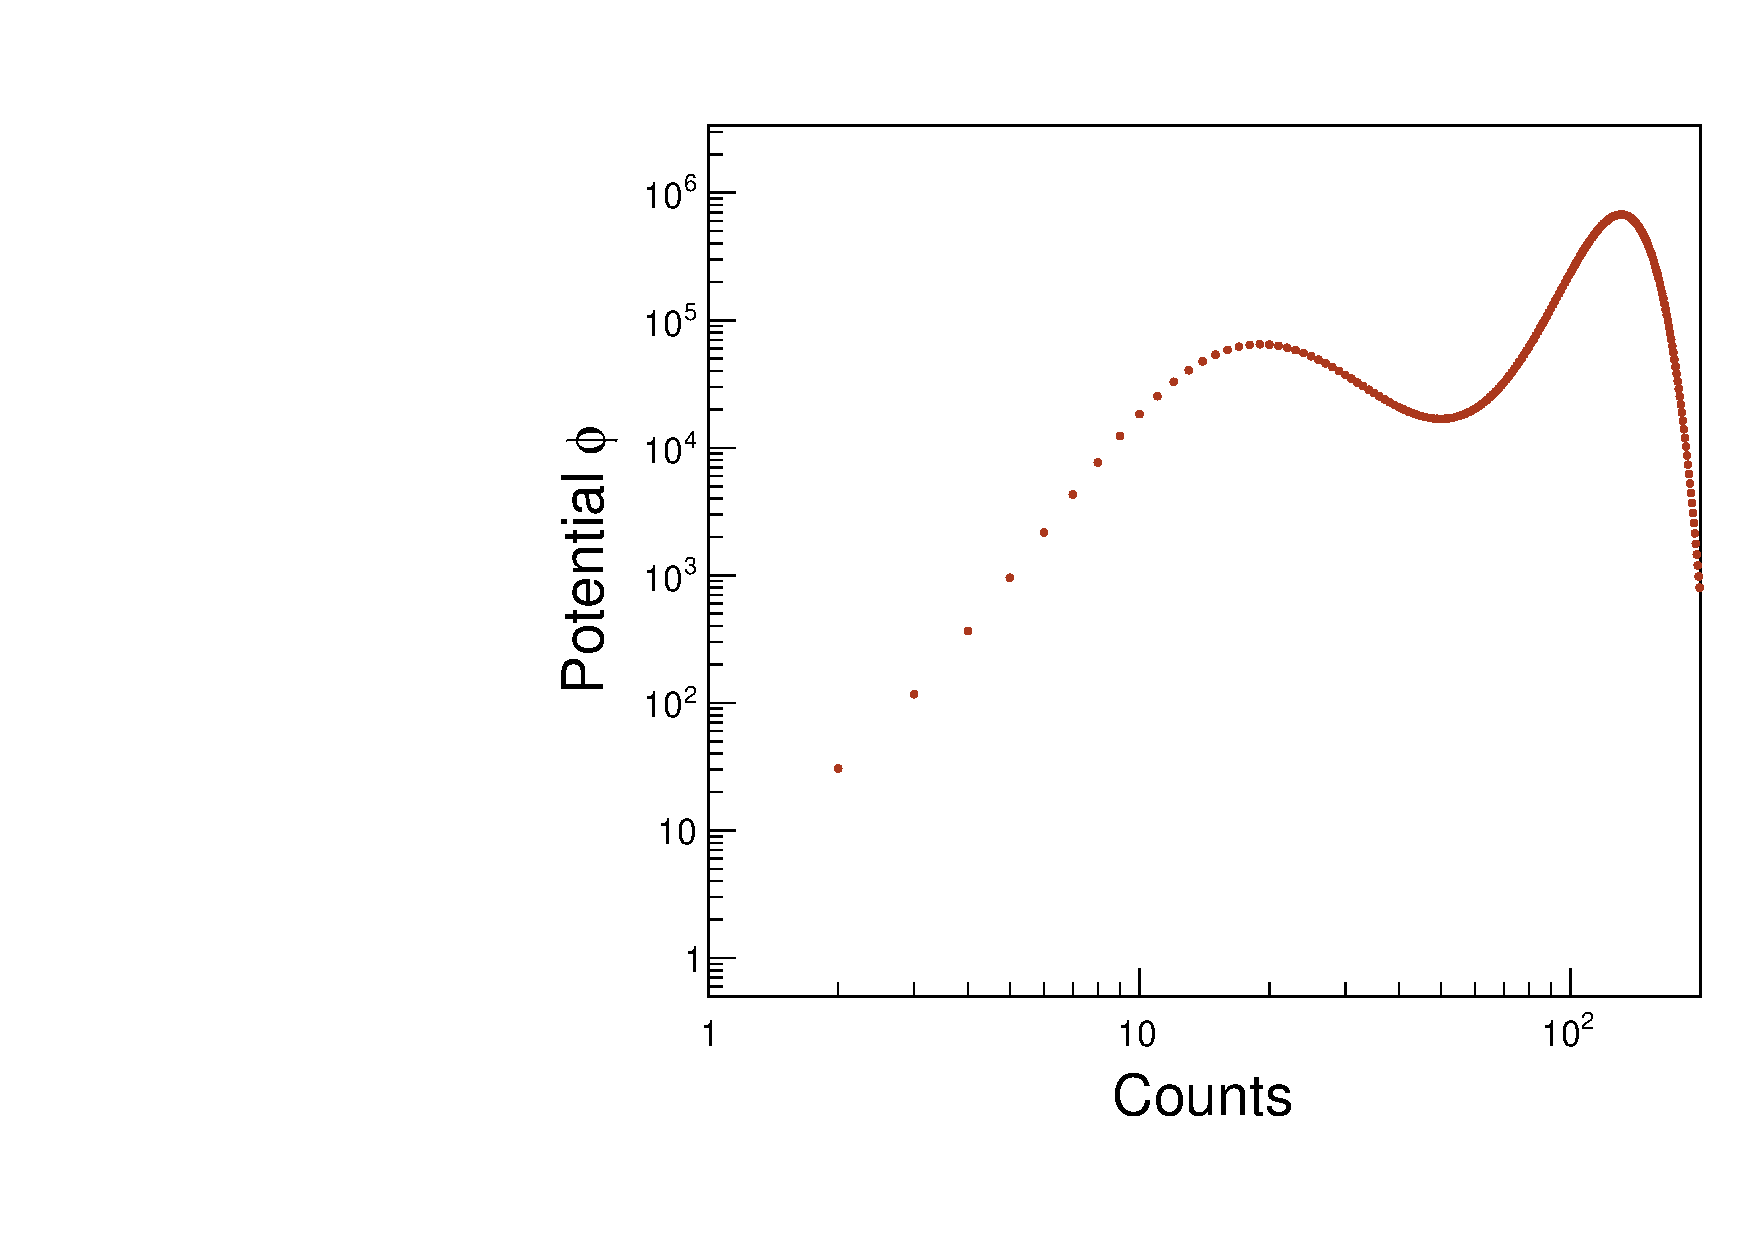
\includegraphics[width=.32\textwidth]{canvPotential_E.pdf} 
    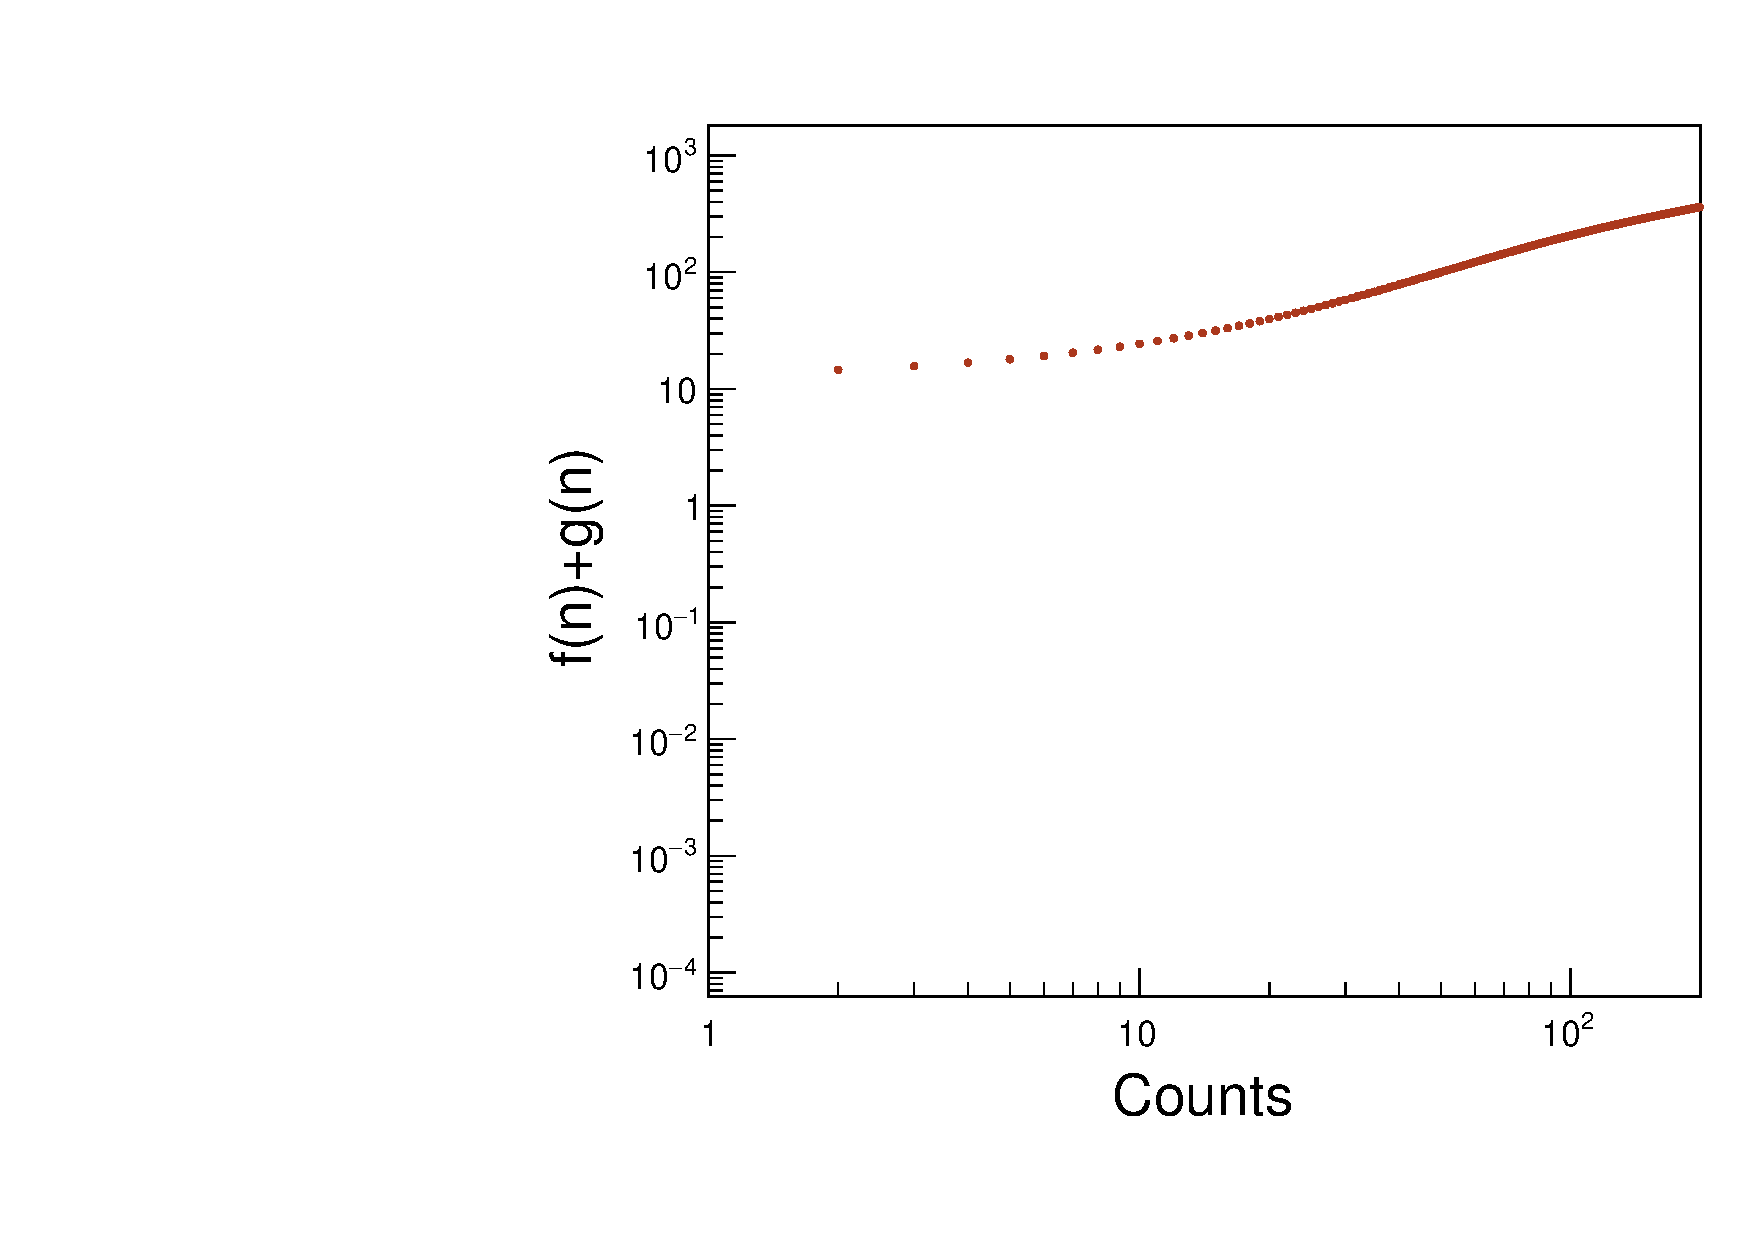
\includegraphics[width=.32\textwidth]{canvPotential_Denom.pdf} 
    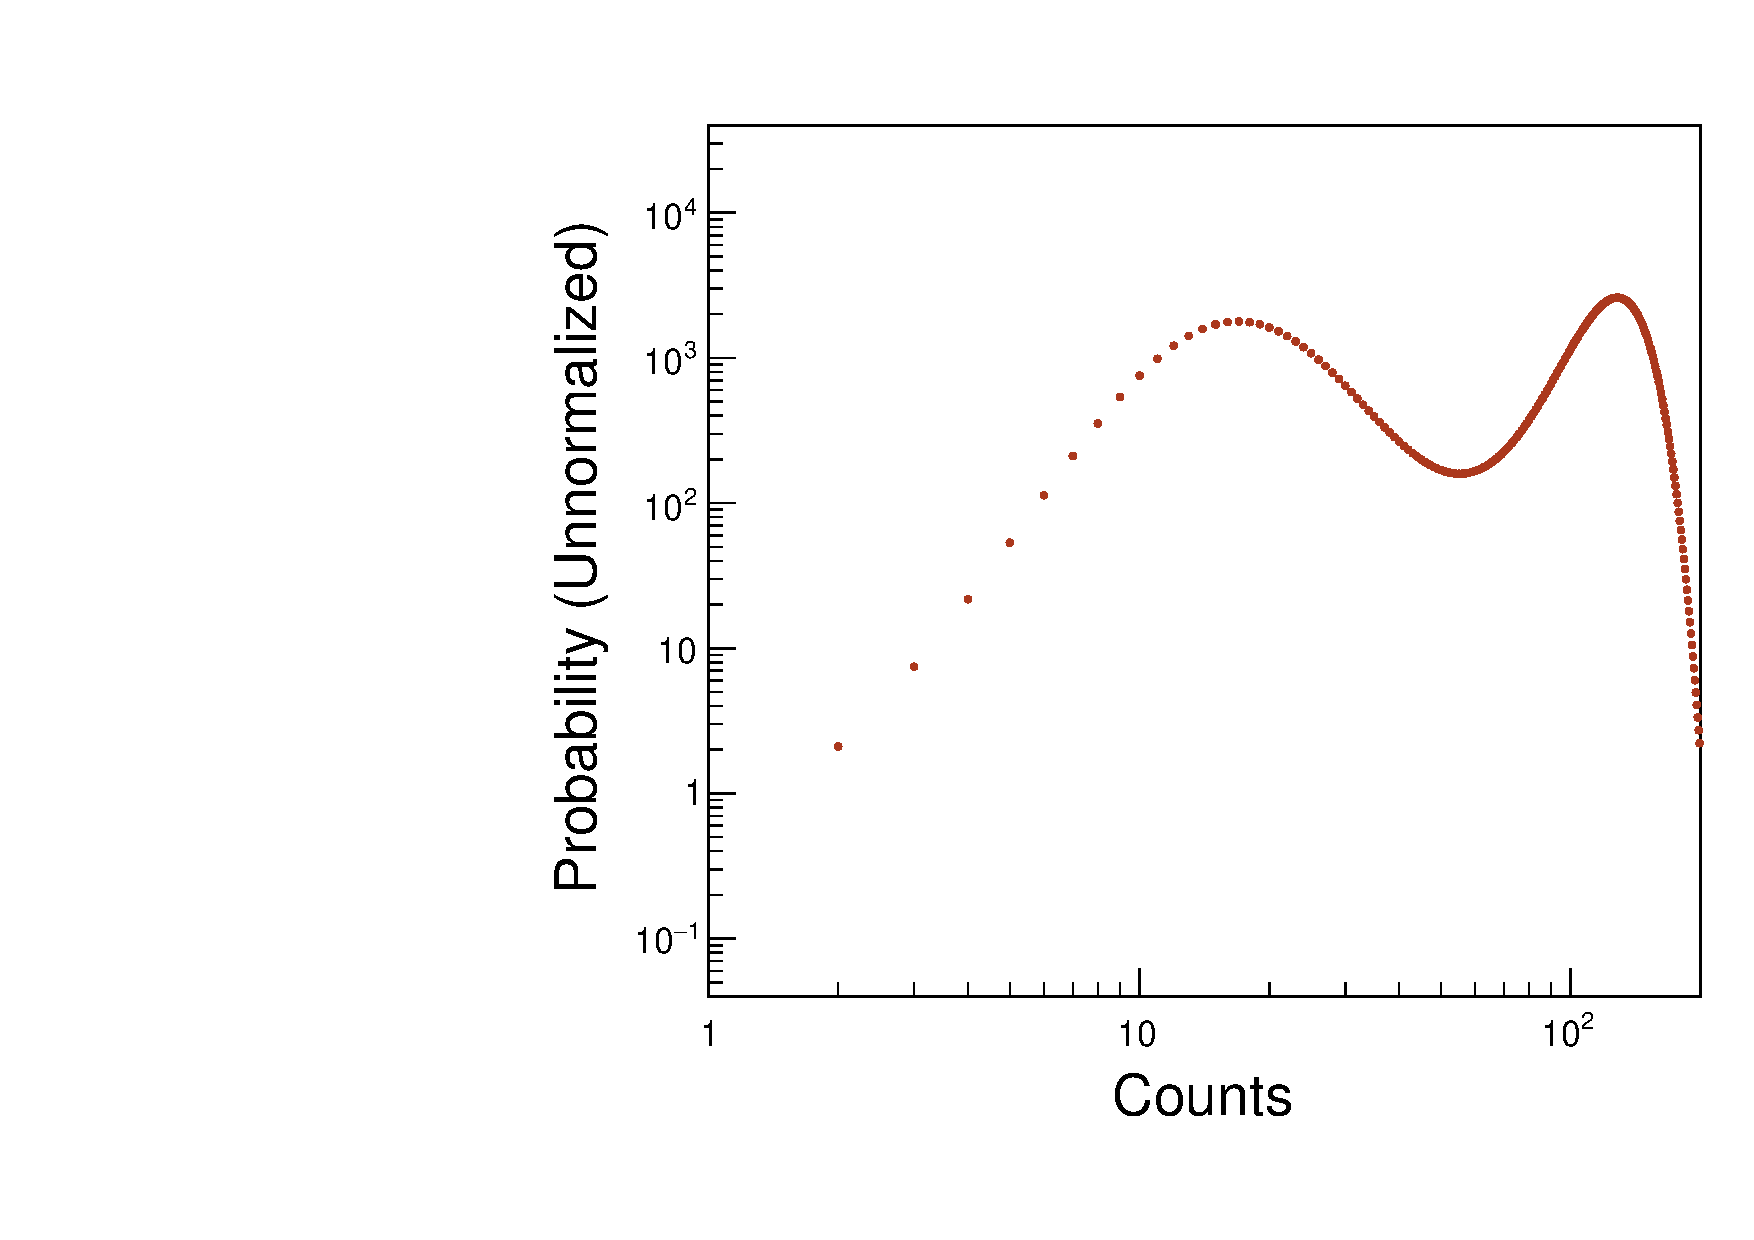
\includegraphics[width=.32\textwidth]{canvPotential_Prob.pdf} 
    \caption{Left to right: exponentiated potential, denominator f(n) + g(n), and the unnormalized probability distribution. The final of these is clearly dominated by the behavior of the exponentiated potential.}
    \label{fig5}
\end{figure}

\begin{figure}[H]
    \centering
    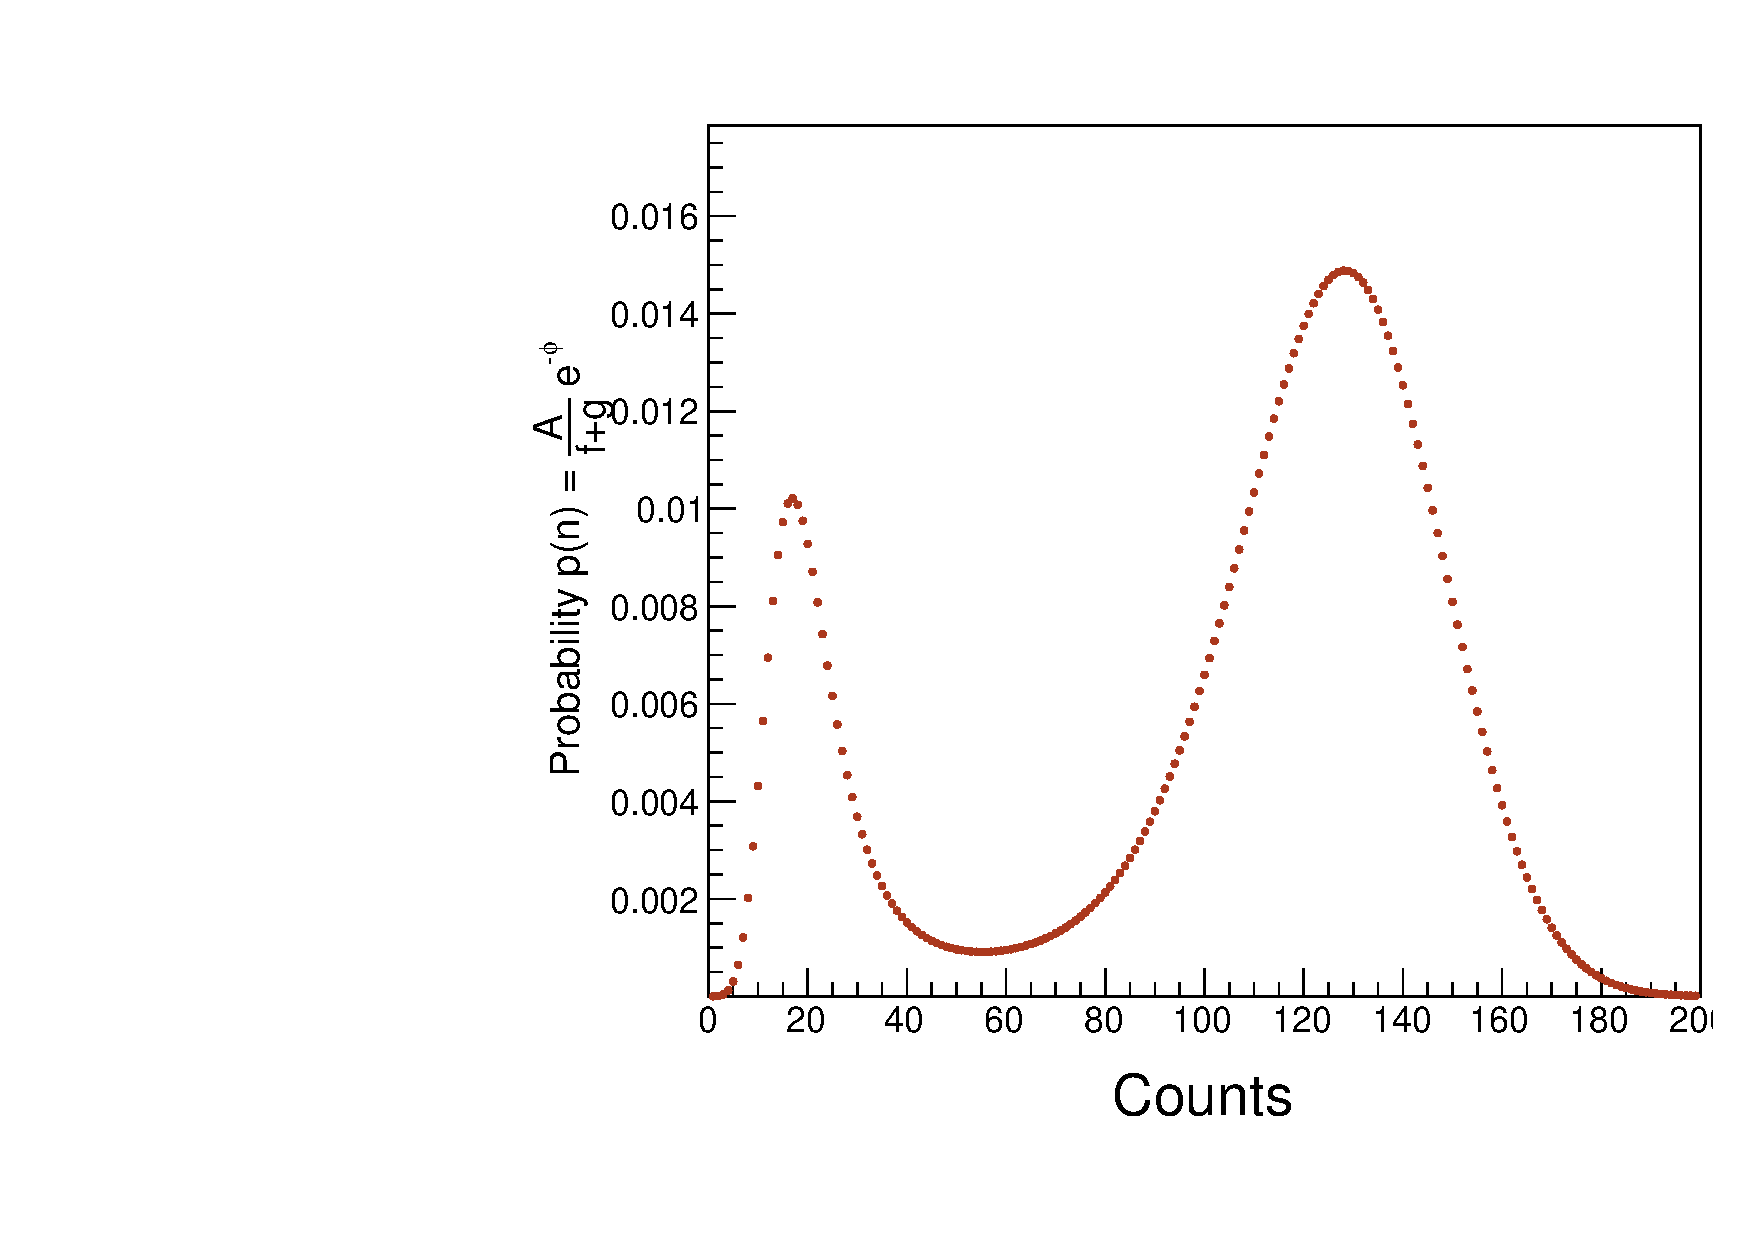
\includegraphics[width=.9\textwidth]{canvPotential_Prob2.pdf} 
    \caption{Normalized probability by value A. Integer steps, summing thru returns 1.}
    \label{fig6}
\end{figure}

\end{document}

